\subsection{Diagrammi delle classi della View}	
		
	\subsubsection{Package Pages}
		\begin{center}
			\centerline{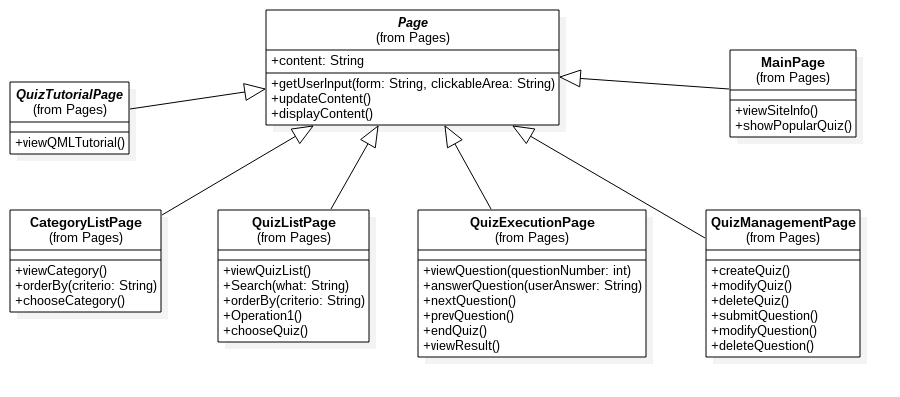
\includegraphics[scale=0.6]{../images/Pages.png}}
		\end{center}
		\subsubsubsection{Interfaccia Page}
			\begin{itemize}
		    		\item\textbf{Funzione del componente:} rappresenta una pagina web
				\item\textbf{Relazioni d'uso di altri componenti:} L'interfaccia Page viene concretizzata dalle sue classi derivate, una rappresentativa per ogni pagina dell'applicazione
				\item\textbf{Attività svolte e dati trattati:} fornisce il contratto di base che una pagina deve soddisfare (visualizzare il proprio contenuto in maniera semplice e fruibile per l'utente). Fornisce inoltre un tipo che gli altri package possono utilizzare per riferirsi ad una qualsiasi pagina indipendentemente dalla sua concretizzazione e favorendo quindi l'estendibilità del codice.
			\end{itemize}
		\subsubsubsection{Classe LoginPage}
			\begin{itemize}
		    		\item\textbf{Funzione del componente:} visualizza il form di autenticazione e permette il login dell'utente. Fornisce inoltre un link alla pagina di registrazione e uno alla pagina di recupero della password 
				\item\textbf{Relazioni d'uso di altri componenti:} concretizza l'interfaccia Page da cui è diretta discendente e utilizza il template LoginForm
				\item\textbf{Attività svolte e dati trattati:} permette l'autenticazione dell'utente nel sistema
			\end{itemize}
		\subsubsubsection{Classe RegistrationPage}
			\begin{itemize}
		    		\item\textbf{Funzione del componente:} visualizza il form di registrazione. Fornisce inoltre un link alla pagina di login
				\item\textbf{Relazioni d'uso di altri componenti:} concretizza l'interfaccia Page da cui è diretta discendente e utilizza il template RegistrationForm
				\item\textbf{Attività svolte e dati trattati:} permette la registrazione dell'utente nel sistema
			\end{itemize}
		\subsubsubsection{Classe PasswordRecoveryPage}
			\begin{itemize}
		  		\item\textbf{Funzione del componente:} visualizza il form per il recupero della password
				\item\textbf{Relazioni d'uso di altri componenti:} concretizza l'interfaccia Page da cui è diretta discendente e utilizza il template PasswordRecoveryForm
				\item\textbf{Attività svolte e dati trattati:} permette il recupero della password dimenticata tramite l'invio di una email
			\end{itemize}
		\subsubsubsection{Classe CategoryListPage}
			\begin{itemize}
		    		\item\textbf{Funzione del componente:} visualizza la lista delle categorie
				\item\textbf{Relazioni d'uso di altri componenti:} concretizza l'interfaccia Page da cui è diretta discendente
				\item\textbf{Attività svolte e dati trattati:} permette la selezione di una categoria che porta ad una pagina in cui vengono visualizzati tutti i questionari della categoria scelta
			\end{itemize}
		\subsubsubsection{Classe QuizListPage}
			\begin{itemize}
		    		\item\textbf{Funzione del componente:} visualizza una lista di questionari
				\item\textbf{Relazioni d'uso di altri componenti:} concretizza l'interfaccia Page da cui è diretta discendente e utilizza il template QuizList
				\item\textbf{Attività svolte e dati trattati:} permette la selezione di un questionario che porta alla pagina di compilazione del questionario scelto
			\end{itemize}
		\subsubsubsection{Classe QuizExecutionPage}
			\begin{itemize}
		    		\item\textbf{Funzione del componente:} visualizza un questionario (una domanda alla volta) e tutti i dati relativi (tempo rimasto, numero domande, ecc...)
				\item\textbf{Relazioni d'uso di altri componenti:} concretizza l'interfaccia Page da cui è diretta discendente e utilizza il template QuestionCompilation
				\item\textbf{Attività svolte e dati trattati:} permette la compilazione di un questionario
			\end{itemize}
		\subsubsubsection{Classe QuizResultsPage}
			\begin{itemize}
		    		\item\textbf{Funzione del componente:} visualizza i risultati del questionario appena compilato
				\item\textbf{Relazioni d'uso di altri componenti:} concretizza l'interfaccia Page da cui è diretta discendente e utilizza il template QuizResults
				\item\textbf{Attività svolte e dati trattati:} permette la compilazione di un questionario
			\end{itemize}
		\subsubsubsection{Classe QuestionManagmentPage}
			\begin{itemize}
		    		\item\textbf{Funzione del componente:} visualizza la lista delle domande create dall'utente
				\item\textbf{Relazioni d'uso di altri componenti:} concretizza l'interfaccia Page da cui è diretta discendente e utilizza il template QuestionList
				\item\textbf{Attività svolte e dati trattati:} permette l'accesso alle pagine di creazione di una nuova domanda e modifica di una domanda esistente. Permette inoltre l'eliminazione di una domanda
			\end{itemize}
		\subsubsubsection{Classe QuestionCreationPage}
			\begin{itemize}
		    		\item\textbf{Funzione del componente:} visualizza il form di creazione di una nuova domanda
				\item\textbf{Relazioni d'uso di altri componenti:} concretizza l'interfaccia Page da cui è diretta discendente e utilizza il template QuestionForm
				\item\textbf{Attività svolte e dati trattati:} permette la creazione di una nuova domanda
			\end{itemize}
		\subsubsubsection{Classe QuestionUpdatePage}
			\begin{itemize}
		    		\item\textbf{Funzione del componente:} visualizza il form di modifica di una domanda
				\item\textbf{Relazioni d'uso di altri componenti:} concretizza l'interfaccia Page da cui è diretta discendente e utilizza il template QuestionForm
				\item\textbf{Attività svolte e dati trattati:} permette la modifica di una domanda
			\end{itemize}
		\subsubsubsection{Classe QuizCreationPage}
			\begin{itemize}
		    		\item\textbf{Funzione del componente:} visualizza il form di creazione di un nuovo questionario
				\item\textbf{Relazioni d'uso di altri componenti:} concretizza l'interfaccia Page da cui è diretta discendente e utilizza il template QuizCreationForm
				\item\textbf{Attività svolte e dati trattati:} permette la creazione di un nuovo questionario
			\end{itemize}
			
	\subsubsection{Package Templates}
		\begin{center}
			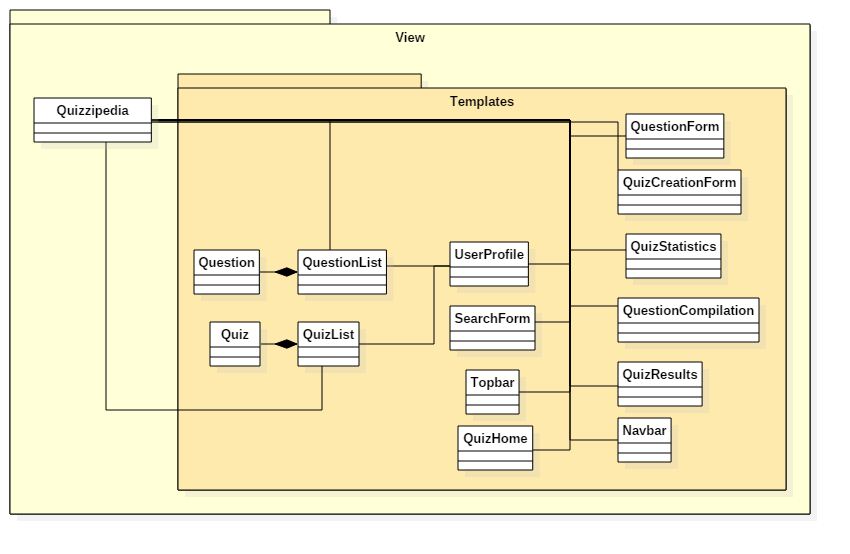
\includegraphics[scale=0.6]{../images/Templates.png}
		\end{center}
		\subsubsubsection{Classe QuestionList}
			\begin{itemize}
				\item\textbf{Funzione del componente:} visualizza una lista di domande
				\item\textbf{Relazioni d'uso di altri componenti:} composta da Question
			\end{itemize}
		\subsubsubsection{Classe Question}
			\begin{itemize}
				\item\textbf{Funzione del componente:} visualizza una domanda inserita in una lista
				\item\textbf{Relazioni d'uso di altri componenti:} usata solo da QuestionList per creare la lista
			\end{itemize}
		\subsubsubsection{Classe QuizList}
			\begin{itemize}
				\item\textbf{Funzione del componente:} visualizza una lista di quiz
				\item\textbf{Relazioni d'uso di altri componenti:} composta da Quiz
			\end{itemize}
		\subsubsubsection{Classe Quiz}
			\begin{itemize}
				\item\textbf{Funzione del componente:} visualizza un quiz inserito in una lista
				\item\textbf{Relazioni d'uso di altri componenti:} usata solo da QuizList per creare la lista
			\end{itemize}
		\subsubsubsection{Classe QuestionCompilation}
			\begin{itemize}
				\item\textbf{Funzione del componente:} visualizza una domanda e ne permette la compilazione
			\end{itemize}
		\subsubsubsection{Classe QuestionForm}
			\begin{itemize}
				\item\textbf{Funzione del componente:} visualizza il form per i dati di una domanda. Utilizzabile sia per la creazione che per la modifica della domanda (se viene modificata una domanda già esistente nei campi vengono inseriti i valori attuali)
			\end{itemize}
		\subsubsubsection{Classe QuizCreation}
			\begin{itemize}
				\item\textbf{Funzione del componente:} visualizza il form di creazione di un questionario
			\end{itemize}
		\subsubsubsection{Classe QuizResults}
			\begin{itemize}
				\item\textbf{Funzione del componente:} visualizza i risultati ottenuti in seguito alla compilazione di un quiz
			\end{itemize}
		\subsubsubsection{Classe SearchForm}
			\begin{itemize}
				\item\textbf{Funzione del componente:} visualizza un form per l'inserimento dei dati desiderati e l'avvio della ricerca
			\end{itemize}
		\subsubsubsection{Classe RegistrationForm}
			\begin{itemize}
				\item\textbf{Funzione del componente:} visualizza un form per la registrazione di un nuovo utente
			\end{itemize}
		\subsubsubsection{Classe LoginForm}
			\begin{itemize}
				\item\textbf{Funzione del componente:} visualizza un form per l'autenticazione di un utente
			\end{itemize}
		\subsubsubsection{Classe PasswordRecoveryForm}
			\begin{itemize}
				\item\textbf{Funzione del componente:} visualizza un form per il recupero della password dimenticata
			\end{itemize}
			
			\newpage